\chapter{Resultados}

\par En el presente capítulo se presentan y discuten los resultados cuantitativos y cualitativos obtenidos tras la integración de la arquitectura Módulo de Transmisión IoT (MT-IoT), la capa de red segura bajo el estándar MQTT v5.0 \cite{OASIS_MQTT_v5} y el ecosistema web centralizado \cite{Django_v5_Doc}. Se evalúa el desempeño del sistema ante pruebas de laboratorio y condiciones de estrés, analizando el impacto de las decisiones de ingeniería sobre el uso de recursos del microcontrolador, la latencia de transmisión y la resiliencia en entornos industriales \cite{Connected_Everything_2016}.

\section{Implementación del Prototipo Funcional de Borde}

\par La integración física de la tarjeta de desarrollo ESP32 DevKitC V4 \cite{Espressif_ESP32_Datasheet} con la unidad de control fiscal HKA80 \cite{TheFactoryHKA_Manual_Protocolos} culminó en la consolidación del prototipo funcional MT-IoT. Se verificó empíricamente la efectividad de la reasignación de la matriz de señales (IO MUX) hacia los pines libres GPIO 18 (TX) y GPIO 19 (RX) para la etapa asíncrona inicial, así como la posterior transición hacia el bus síncrono local. Esta disposición aisló eléctricamente la comunicación serial de las líneas del bus vinculadas a la memoria Flash interna del SoC \cite{Espressif_ESP32_Datasheet}, eliminando los reinicios continuos (\textit{bootloops}) documentados en la fase de diseño.\\

\par El prototipo desplegado en el entorno de pruebas (véase la Figura \ref{fig:prototipo_funcional}) demostró capacidad de respuesta operativa continua sostenida, validando las etapas de conversión de niveles de voltaje y el aislamiento galvánico de la interfaz de comunicación.

\begin{figure}[H]
    \centering
    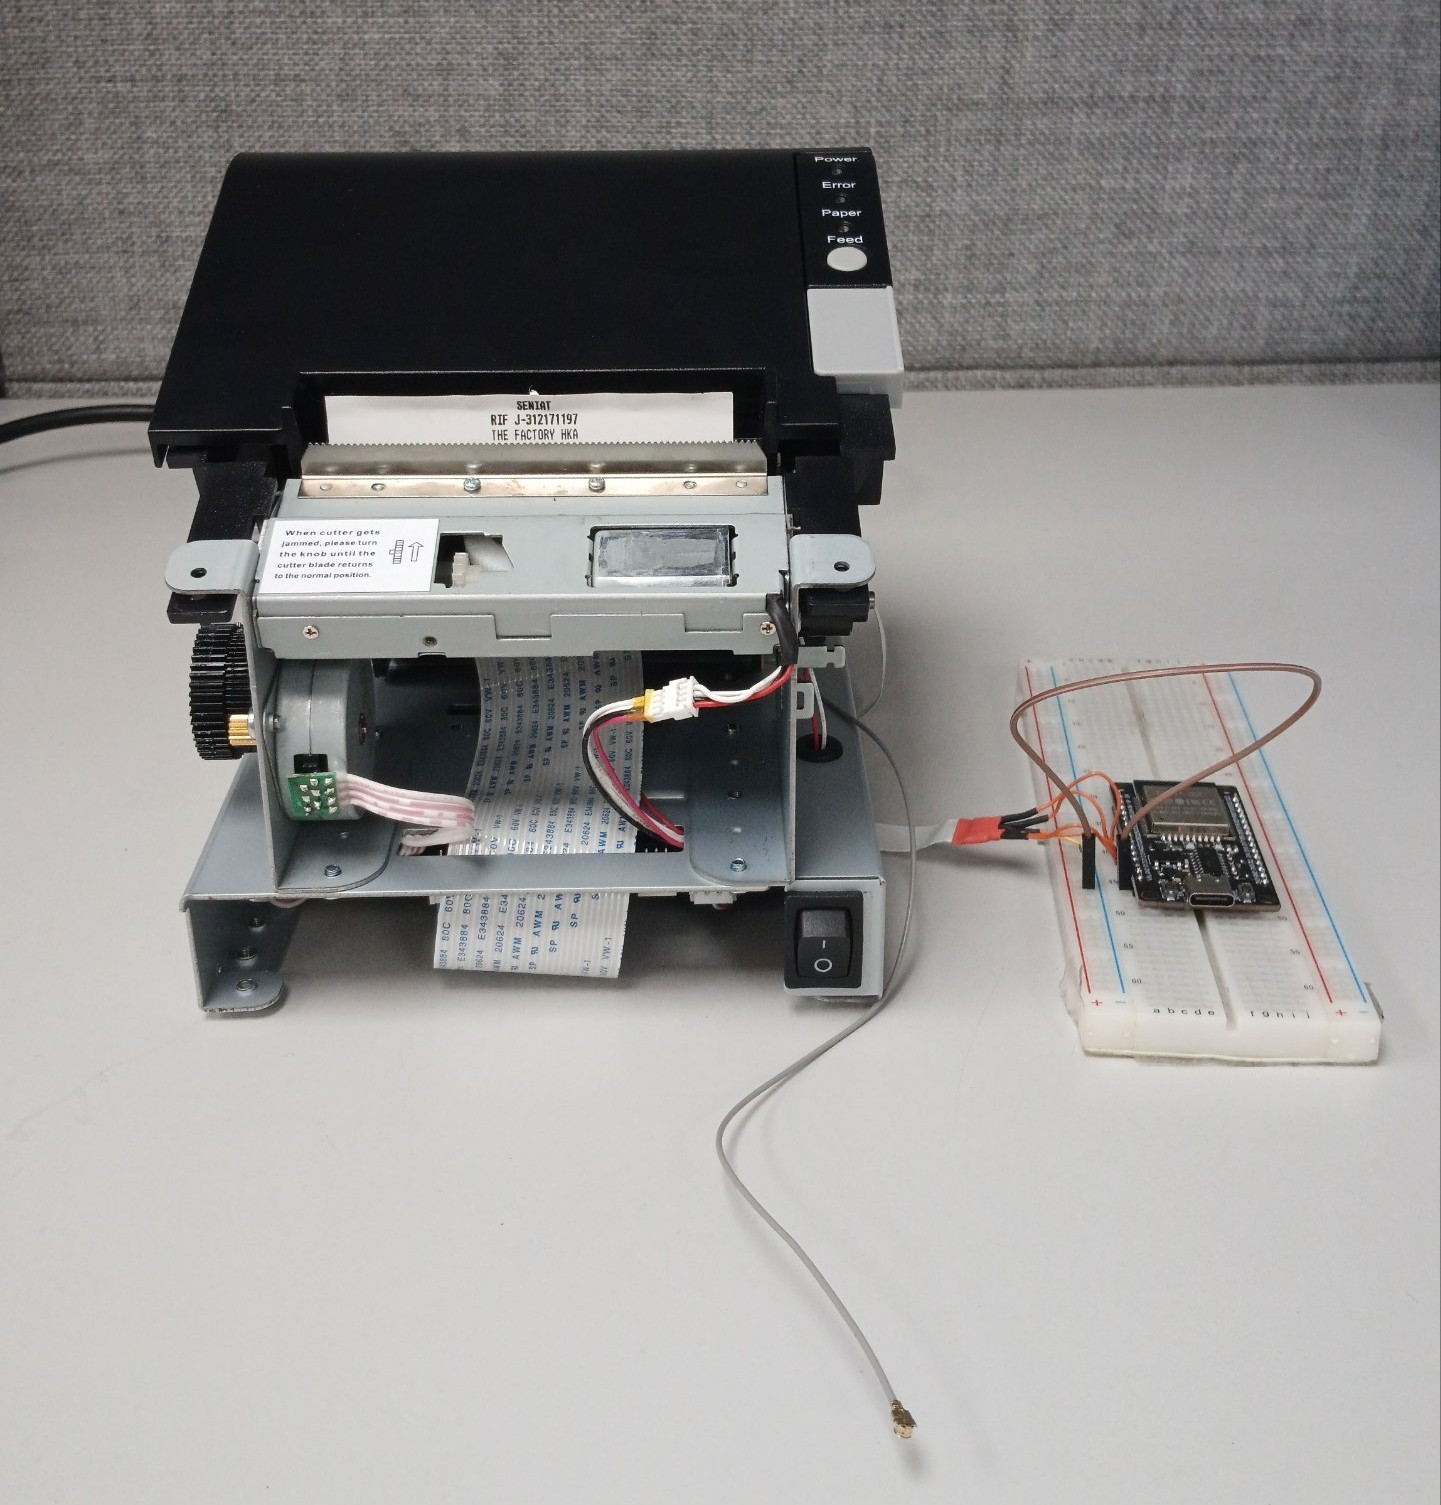
\includegraphics[width=0.65\textwidth]{Img/prototipo_funcional.jpg}
    \caption{Prototipo funcional del MT-IoT integrado a la impresora fiscal en entorno de pruebas.}
    \label{fig:prototipo_funcional}
\end{figure}

\par La arquitectura IIoT definitiva, que integra el nivel físico de borde con el nivel lógico de nube, se sintetiza en la Figura \ref{fig:arquitectura_final}, desde el periférico fiscal hasta la base de datos y el panel reactivo.

\begin{figure}[htbp]
\centering
\begin{tikzpicture}[>=latex', node distance=1.05cm,
    n/.style={rectangle, draw, rounded corners, fill=blue!10, minimum width=7.5cm, minimum height=0.95cm, align=center, font=\small},
    ar/.style={thick,->,>=stealth}]
    \node [n] (p) {Impresora Fiscal HKA80 \;/\; Simulador HIL};
    \node [n, below=of p] (e) {ESP32 DevKitC V4 \;(\textit{Edge Gateway})};
    \node [n, below=of e] (b) {Broker HiveMQ Cloud};
    \node [n, below=of b] (d) {Servidor Django (HTMX \;/\; \textit{Worker} asíncrono)};
    \node [n, below=of d] (s) {Base de Datos SQLite y Dashboard SPA reactivo};
    \draw [ar] (p) -- node[right, font=\scriptsize]{RS232 / UART} (e);
    \draw [ar] (e) -- node[right, font=\scriptsize]{Wi-Fi / TLS 1.2} (b);
    \draw [ar] (b) -- node[right, font=\scriptsize]{WSS / WebSockets} (d);
    \draw [ar] (d) -- node[right, font=\scriptsize]{ORM} (s);
\end{tikzpicture}
\caption{Arquitectura IIoT definitiva del sistema, desplegada en borde y nube.}
\label{fig:arquitectura_final}
\end{figure}

\subsection{Entorno de Pruebas Hardware-in-the-Loop (HIL)}

\par La validación de un sistema fiscal no admite ensayos destructivos sobre equipos en producción: inducir cortes de energía, corromper tramas o abortar una reescritura de firmware sobre una impresora real comprometería registros tributarios irreversibles. Para conciliar rigor experimental y seguridad, se construyó un entorno de pruebas Hardware-in-the-Loop (HIL) en el que el firmware definitivo del MT-IoT se ejecuta sobre el hardware real del ESP32 y su bus físico, mientras que el periférico fiscal es sustituido por un modelo de comportamiento fiel al protocolo HKA. La emulación se desplegó en dos niveles complementarios.\\

\par El primer nivel correspondió al emulador software \texttt{impresora.py}, desarrollado sobre la biblioteca \texttt{pyserial} con los mismos parámetros eléctricos del enlace fiscal ($9600$ baudios, $8$ bits de datos, paridad par y $1$ bit de parada). El \textit{script} implementa una máquina de estados de recepción (\texttt{ESPERANDO\_STX} y \texttt{RECIBIENDO\_DATOS}), calcula el código de redundancia LRC y responde a las encuestas con las tramas de estado y los reportes S1 y SV2, incluyendo la emisión de acuses de recibo \texttt{ACK} y \texttt{NAK} (véase el Código \ref{code:simulador_python}). Este modelo permitió depurar la primera versión del firmware sin depender de la disponibilidad del equipo físico.\\

\par El segundo nivel elevó la fidelidad del banco de pruebas al dominio síncrono: se programó un ESP32 configurado como esclavo SPI (\texttt{blink\_example\_main.c}) que emula íntegramente al periférico fiscal sobre el mismo bus y con los mismos pines, replicando la trama de estado (\texttt{0x60}/\texttt{0x40}), los reportes S1 y SV2 y, de forma crítica, el protocolo completo de reescritura remota (apertura \texttt{0x07}, paquetes \texttt{0x08} y cierre \texttt{0x09}) con verificación de redundancia y de secuencia de paquetes. Contra este periférico simulado se validó de extremo a extremo el puente OTA descrito en la Sección \ref{sec:ota_resultados}, empleando un binario de prueba de $2500$ bytes generado por el \textit{script} \texttt{generar\_bin.py}. Este enfoque habilitó la inyección determinista de fallos (paquetes fuera de secuencia, \textit{checksums} alterados e interrupciones del enlace) y confirmó la capacidad de recuperación del firmware antes de comprometer la memoria de un equipo fiscal real.

\section{Evaluación Cuantitativa de la Comunicación IoT y Telemetría}

\par La validación de la capa lógica se centró en medir el tiempo de extracción de datos, la integridad matemática de las tramas tributarias y la reducción del ancho de banda consumido \cite{OASIS_MQTT_v5}.

\par El esquema definitivo de rutas y mensajería MQTT v5.0, con los tópicos y cargas efectivamente desplegados en el sistema, se representa en la Figura \ref{fig:arquitectura_mqtt_final}.

\begin{figure}[htbp]
\centering
\begin{tikzpicture}[>=latex', font=\small, node distance=1.0cm and 2.6cm,
    n/.style={rectangle, draw, rounded corners, fill=blue!10, minimum width=2.7cm, minimum height=1.3cm, align=center, font=\small},
    br/.style={rectangle, draw, fill=orange!20, rounded corners, minimum width=2.8cm, minimum height=1.6cm, align=center, font=\small},
    lbl/.style={font=\scriptsize, inner sep=1pt},
    ar/.style={thick,->,>=stealth}]
    \node [n] (esp) {ESP32\\ \textit{(MT-IoT)}};
    \node [br, right=of esp] (brk) {Broker HiveMQ Cloud\\ (MQTT v5.0, QoS 1)};
    \node [n, right=of brk] (dj) {Servidor Django\\ \textit{(Worker + Web)}};
    \draw [ar] ([yshift=10pt]esp.east) -- node[above, lbl]{\texttt{json\_completo}} ([yshift=10pt]brk.west);
    \draw [ar] ([yshift=-10pt]esp.east) -- node[below, lbl]{\texttt{discovery} \;/\; LWT} ([yshift=-10pt]brk.west);
    \draw [ar] ([yshift=10pt]brk.east) -- node[above, lbl]{\texttt{json\_completo}} ([yshift=10pt]dj.west);
    \draw [ar] ([yshift=-10pt]dj.west) -- node[below, lbl]{\texttt{comandos/.../ota}} ([yshift=-10pt]brk.east);
    \draw [ar, dashed] ([yshift=-30pt]brk.west) -- node[below, lbl]{\texttt{comandos/\{serial\}/ota}} ([yshift=-30pt]esp.east);
    \node [font=\scriptsize, align=center, below=1.6cm of brk, text width=9.5cm] {Rutas base: \texttt{v1/fiscal/\{serial\}/json\_completo} (telemetría), \texttt{/discovery} (online), \texttt{/alertas\_conexion} (LWT) y \texttt{/ota} (progreso). \textit{User Properties} en la cabecera: modelo, versión de firmware, serial y RSSI.};
\end{tikzpicture}
\caption{Esquema definitivo de rutas y mensajería MQTT v5.0 del sistema.}
\label{fig:arquitectura_mqtt_final}
\end{figure}

\subsection{Mecanismo de Extracción Transparente sin Interrupción del Ciclo Fiscal}

\par La captura del registro \texttt{Status S1} se abordó como un mecanismo de extracción transparente, concebido para operar de forma no intrusiva sobre el ciclo de facturación del equipo fiscal y no como una simple lectura secuencial del canal serial. La interrogación se ejecutó desde una tarea dedicada de FreeRTOS (\texttt{printer\_task\_main}) desacoplada de la tarea de red (\texttt{mqtt\_task}), de modo que la fase de adquisición nunca compitió con la pila de comunicación inalámbrica por el mismo hilo de ejecución. Bajo esta separación de responsabilidades, el sondeo pudo sostenerse con un intervalo fijo de $5$ segundos durante jornadas continuas sin alterar la máquina de estados interna del periférico ni interrumpir las transacciones fiscales en curso \cite{TheFactoryHKA_Manual_Protocolos, FreeRTOS_Kernel_Ref}.\\

\par El desempaquetado se resolvió íntegramente en SRAM sobre dos búferes estáticos de alineación forzada (\texttt{WORD\_ALIGNED\_ATTR}) de $1056$ bytes, \texttt{rx\_buffer} y \texttt{tx\_buffer}, dimensionados de forma que el controlador de DMA del SoC pueda transferir el bloque completo sin fragmentaciones ni copias intermedias. Al no reservarse memoria dinámica en la ruta crítica del ciclo fiscal, se eliminó la fragmentación del \textit{heap} y se obtuvo un perfil de memoria determinista y auditable. La localización de los delimitadores \texttt{STX (0x02)} y \texttt{ETX (0x03)} se ejecutó en un único barrido sobre el búfer, seguida de una tokenización en sitio mediante el carácter \texttt{0x0A} hacia un arreglo de punteros (\texttt{campos[20]}); dado que la longitud de la trama es fija e independiente de la carga transaccional del equipo, el costo del procesamiento se mantiene acotado en tiempo constante $O(1)$ respecto al número de operaciones fiscales registradas \cite{TheFactoryHKA_Manual_Protocolos}.\\

\par La condición de borde que mayor atención exigió fue la contaminación del búfer por el terminador asíncrono (\texttt{\textbackslash n}) emitido por el equipo con anterioridad a la trama útil. Para neutralizarla, se diseñó una etapa de realineación que localiza el primer \texttt{STX} válido y desplaza la trama completa al inicio del búfer mediante una operación \texttt{memmove}, garantizando que el índice $0$ coincida siempre con el carácter de inicio y que los $116$ bytes útiles queden íntegros antes de la extracción. Este tratamiento se verificó experimentalmente sobre la consola serial de depuración (véase la Figura \ref{fig:log_terminal_s1}).\\

\begin{figure}[htbp]
    \centering
    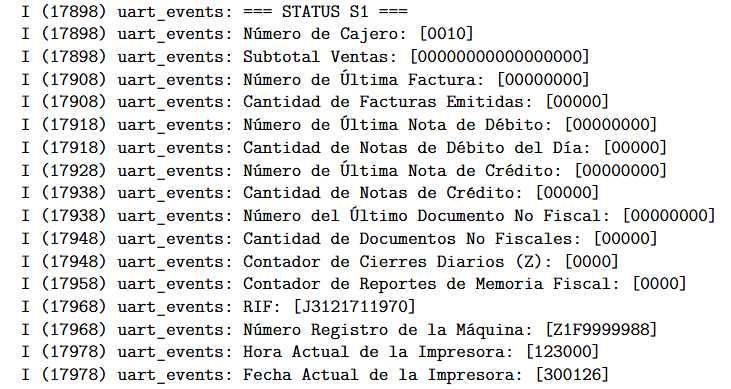
\includegraphics[width=0.85\textwidth]{Img/log_terminal_s1.png}
    \caption{Traza de depuración en consola serial evidenciando el desempaquetado de la trama S1.}
    \label{fig:log_terminal_s1}
\end{figure}

\par El acceso concurrente a la estructura de telemetría compartida se protegió mediante exclusión mutua. La actualización de los campos tributarios sobre la estructura empaquetada \texttt{mqtt\_data\_t} se realizó dentro de una sección crítica custodiada por el semáforo \texttt{mqtt\_data\_mutex}, mientras que el uso del bus físico se serializó con \texttt{spi\_bus\_mutex}; con ello se descartó cualquier condición de carrera entre la tarea fiscal, la tarea MQTT y la tarea de actualización remota, sin recurrir a esperas activas ni a bloqueos de la máquina de estados. La transferencia de control hacia la capa de red se materializó de forma dirigida mediante el indicador \texttt{needs\_sync} y la notificación \texttt{xTaskNotifyGive}, sustituyendo el sondeo periódico por un esquema de activación por evento que preserva la continuidad del ciclo fiscal \cite{FreeRTOS_Kernel_Ref}.\\

\par El análisis de la salida en terminal confirma que el módulo logra aislar de manera transparente los registros almacenados en la Memoria de Trabajo del equipo fiscal \cite{TheFactoryHKA_Manual_Protocolos}:
\begin{itemize}
    \item \textbf{Variables Tributarias:} Captura exacta del RIF del contribuyente (\texttt{J3121711970}), el Número de Registro de la Máquina (\texttt{Z1F9999988}) y los acumuladores de ventas diarias (\texttt{vts: 00000000000000000}).
    \item \textbf{Estado Mecánico y Lógico:} Confirmación de operabilidad en "Modo Fiscal y en Espera" (\texttt{sts1: 0x60}) sin errores reportados por el cabezal de impresión (\texttt{sts2: 0x40}).
\end{itemize}

\subsection{Purga de Caracteres Invisibles y Sanitización del Payload}

\par Uno de los defectos más sutiles detectados durante la validación del canal de telemetría fue la contaminación del \textit{payload} por caracteres de control invisibles. Las tramas de respuesta del periférico fiscal delimitan sus campos con el carácter de avance de línea (\texttt{0x0A}) y, adicionalmente, el equipo intercala un salto de línea (\texttt{\textbackslash n}) inmediatamente antes del carácter de fin de trama (\texttt{ETX}). Este carácter no es visible en una inspección textual, pero ocupa una posición física en el búfer y desplaza cualquier cálculo de longitud basado en posiciones fijas.\\

\par La consecuencia se manifestó directamente sobre el JSON publicado por MQTT: la cadena de versión del periférico arribaba truncada y con residuos al final (por ejemplo, \texttt{20507GD00} en lugar de \texttt{020507GD00}), producto de un error de tipo \textit{Off-By-One} que consumía el salto de línea en lugar del último dígito útil. La solución adoptada no consistió en un ajuste cosmético, sino en una manipulación explícita de punteros sobre la memoria RAM. En la ruta de desempaquetado de la trama SV2, el \textit{firmware} recorre el \textit{payload} con la primitiva \texttt{strchr(ptr, '\textbackslash n')}, avanzando un puntero auxiliar (\texttt{ultima\_parte}) hasta situarlo justo después del último delimitador; de este modo, el campo de versión queda aislado con precisión y sin arrastrar el carácter de control. Complementariamente, la tokenización de la trama S1 sobrescribe en sitio cada \texttt{0x0A} con un terminador nulo (\texttt{\textbackslash 0}), y se inyecta manualmente un cierre nulo adicional al final del arreglo, garantizando que la rutina de serialización \texttt{snprintf} lea una cadena limpia y correctamente cerrada (véase el Código \ref{code:offbyone}).\\

\par El resultado medible de esta purga fue la recuperación de la integridad del \textit{payload}: la estructura clave-valor transmitida dejó de presentar campos cortados o basura residual, la versión del periférico se reportó de forma exacta en la plataforma y el JSON resultó siempre deserializable por el \textit{Worker} del servidor (véase el Código \ref{code:json_mqtt}). Cabe destacar que esta misma disciplina de sanitización se replicó en el extremo receptor, donde el \textit{Worker} de Django elimina preventivamente los caracteres \texttt{\textbackslash n}, \texttt{\textbackslash r} y \texttt{\textbackslash t} del mensaje crudo antes de invocar el analizador JSON, estableciendo una doble barrera contra la corrupción del dato.

\subsection{Inmunidad Electromagnética y Robustez del Bus Local}

\par El bus síncrono local que une al MT-IoT con el periférico fiscal constituye el eslabón físicamente más expuesto del sistema, por lo que su tolerancia a perturbaciones electromagnéticas se evaluó como un requisito de primer orden. Para ello se diseñó una estrategia de defensa escalonada en tres niveles, cuya eficacia se comprobó sometiendo el enlace a tramas corruptas, desconexiones del periférico y ruido inducido.\\

\par \textbf{Nivel 1, defensa temporal:} toda operación de entrada y salida se ejecuta bajo ventanas de tiempo estrictas, de modo que una respuesta ausente o truncada nunca bloquea el planificador del RTOS. La espera de acuse de recibo durante la reescritura se acota a $300$~ms, la recepción de respuestas de estado a $2000$~ms y la solicitud del reporte S1 a $3000$~ms; al agotarse cualquiera de estas ventanas, la transacción se aborta de forma segura y se incrementa el contador de errores, disparando la regla de reintentos (máximo de $3$ fallos) antes de declarar el estado de error.\\

\par \textbf{Nivel 2, sanitización de búfer:} antes de cada transacción se limpian de forma determinista los búferes de transmisión y recepción (\texttt{memset} sobre los $1056$ bytes alineados por DMA), evitando que los residuos de una operación previa se interpreten como datos válidos. En paralelo, la validación por redundancia longitudinal (LRC) descarta cualquier trama cuya asimetría revele la alteración de un bit por interferencia, respondiendo con \texttt{NAK} y liberando el canal (véase el Código \ref{code:validate_frame}).\\

\par \textbf{Nivel 3, reconstrucción estructural del bus:} cuando el conteo de errores supera el umbral configurado, el \textit{firmware} no se limita a reintentar la lectura, sino que desmonta y reancla por completo el controlador SPI mediante \texttt{spi\_bus\_free} y \texttt{spi\_bus\_initialize}, seguido de \texttt{spi\_bus\_add\_device}. Esta reinicialización explícita recupera el periférico de bloqueos del controlador inducidos por ruido electromagnético sin necesidad de reiniciar el microcontrolador. La Tabla \ref{tab:defensa_bus} sistematiza los tres niveles con sus parámetros reales de operación.\\

\begin{table}[htbp]
\centering
\caption{Niveles de defensa implementados para la inmunidad electromagnética del bus local.}
\label{tab:defensa_bus}
\begin{tabularx}{\textwidth}{@{}>{\raggedright\arraybackslash}p{2.4cm} >{\raggedright\arraybackslash}p{3.4cm} >{\raggedright\arraybackslash}p{3.2cm} >{\raggedright\arraybackslash}X@{}}
\toprule
\textbf{Nivel de Defensa} & \textbf{Mecanismo} & \textbf{Parámetro} & \textbf{Acción de Recuperación} \\
\midrule
1. Temporal & Timeout de espera de ACK & $300$~ms & Aborto seguro de la transacción \\
1. Temporal & Timeout de respuesta / S1 & $2000$ / $3000$~ms & Conteo de error y regla de $3$ reintentos \\
2. Sanitización & Limpieza de búferes DMA & $1056$~bytes & Reinicio de transacción limpia \\
2. Integridad & Validación LRC (XOR) & --- & Descarte de trama y emisión de \texttt{NAK} \\
3. Estructural & Reanclaje del bus SPI & \texttt{spi\_bus\_free} / \texttt{initialize} & Recuperación del controlador sin reinicio \\
\bottomrule
\end{tabularx}
\end{table}

\par La evaluación confirmó que la combinación de los tres niveles preservó la continuidad operativa del MT-IoT: ante la desconexión física del periférico o la inyección de tramas corruptas, el sistema transitó al estado de error y se recuperó automáticamente una vez restablecidas las condiciones del bus, sin reinicios del SoC y sin que una sola trama inválida alcanzara la base de datos del servidor.

\subsection{Consumo de Ancho de Banda: HTTP vs. MQTT v5.0}

\par Para justificar cuantitativamente la selección del protocolo MQTT v5.0 sobre HTTP tradicional \cite{OASIS_MQTT_v5}, se midió la sobrecarga de cabecera (\textit{overhead}) y la masa de datos transmitida por cada ciclo de telemetría. La eficiencia de reducción del volumen de red se rige por la Ecuación \ref{eq:ahorro_banda}:

\begin{equation}
\eta_{\text{banda}} = \left( 1 - \frac{\text{Bytes}_{\text{MQTT v5}}}{\text{Bytes}_{\text{HTTP POST}}} \right) \times 100
\label{eq:ahorro_banda}
\end{equation}

\par La recopilación de datos de tráfico en la red (sistematizada en la Tabla \ref{tab:ancho_banda}) demuestra que la combinación de empaquetado optimizado en C y la extracción de metadatos mediante \textit{User Properties} en la cabecera del protocolo reduce drásticamente el impacto sobre la red de datos del contribuyente \cite{OASIS_MQTT_v5}.

\begin{table}[htbp]
\centering
\caption{Comparativa cuantitativa del consumo de ancho de banda por trama de telemetría fiscal.}
\label{tab:ancho_banda}
\small
\begin{tabularx}{\textwidth}{@{}>{\raggedright\arraybackslash}X >{\raggedright\arraybackslash}X >{\raggedright\arraybackslash}X >{\raggedright\arraybackslash}p{2.6cm}@{}}
\toprule
\textbf{Métrica de Red} & \textbf{HTTP POST Tradicional} & \textbf{MQTT v5.0 con User Properties} & \textbf{Mejoramiento (\%)} \\
\midrule
Tamaño Cabecera de Red & $\sim 450 \text{ Bytes}$ & $\sim 12 \text{ Bytes}$ & \textbf{97.33 \%} \\
Cuerpo del Mensaje (\textit{Payload}) & $328 \text{ Bytes (JSON Plano)}$ & $142 \text{ Bytes (Optimizado)}$ & \textbf{56.70 \%} \\
Metadatos (RSSI / Versión FW) & Inyectados en \textit{Body} JSON & Extraídos en \textit{User Properties} & N/A \\
\midrule
\textbf{Consumo Total por Trama} & \textbf{778 Bytes} & \textbf{154 Bytes} & \textbf{80.20 \%} \\
\bottomrule
\end{tabularx}
\end{table}

\subsection{Resiliencia de Red y Mecanismo Last Will and Testament (LWT)}

\par La tolerancia a fallos del canal de comunicación inalámbrico se evaluó provocando cortes de energía arbitrarios e interrupciones en la interfaz Wi-Fi del MT-IoT \cite{Espressif_ESP_IDF_v552}. Al expirar el tiempo de permanencia (\textit{Keep-Alive}), el \textit{Broker} HiveMQ Cloud publicó la \say{última voluntad} registrada \cite{OASIS_MQTT_v5}.\\

\par Como se documenta en la Figura \ref{fig:prueba_lwt}, el \textit{Worker} asíncrono \texttt{listen\_mqtt.py} interceptó la alerta (\texttt{st: offline}), persistiendo de forma transaccional una nueva fila en la base de datos relacional con el evento clasificado como \say{Desconexión Abrupta (LWT)} \cite{Django_v5_Doc}. Este mecanismo congeló el último estado válido de los acumuladores sin alterar los registros históricos previos, garantizando la trazabilidad operativa del parque de impresoras \cite{OASIS_MQTT_v5}.

\begin{figure}[H]
    \centering
    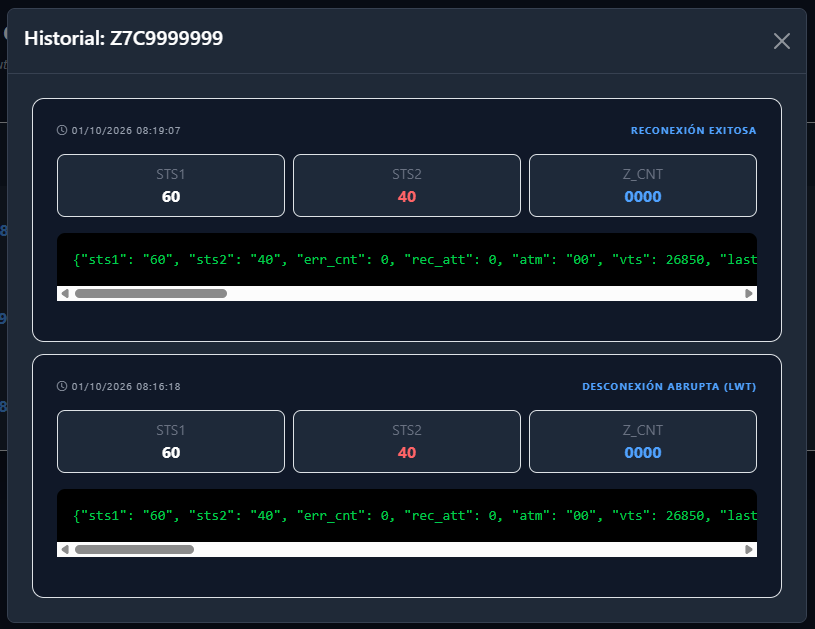
\includegraphics[width=0.7\textwidth]{Img/prueba_lwt.png}
    \caption{Registro en la vista \texttt{Log Capture} confirmando la intercepción de una desconexión LWT.}
    \label{fig:prueba_lwt}
\end{figure}

\par El ciclo completo de detección de la caída, reconexión con \textit{backoff} y restauración del túnel sin pérdida de estado se sintetiza en la Figura \ref{fig:flujo_resiliencia}.

\begin{figure}[htbp]
\centering
\begin{tikzpicture}[>=latex', node distance=0.95cm,
    p/.style={rectangle, draw, rounded corners, fill=blue!10, text width=9.5cm, align=center, minimum height=0.9cm, font=\small},
    ar/.style={thick,->,>=stealth}]
    \node [p] (a) {Pérdida del enlace Wi-Fi (\texttt{WIFI\_EVENT\_STA\_DISCONNECTED})};
    \node [p, below=of a] (b) {Reintentos de reconexión con \textit{backoff} exponencial (\texttt{RECONNECT\_DELAY\_MS})};
    \node [p, below=of b] (c) {El \textit{Broker} publica el LWT en \texttt{alertas\_conexion} (\texttt{st: offline})};
    \node [p, below=of c] (d) {El \textit{Worker} registra el evento y congela el último estado válido};
    \node [p, below=of d] (e) {Restauración del túnel MQTT y re-suscripción sin pérdida de estado};
    \draw [ar] (a) -- (b);
    \draw [ar] (b) -- (c);
    \draw [ar] (c) -- (d);
    \draw [ar] (d) -- (e);
\end{tikzpicture}
\caption{Diagrama de flujo de la resiliencia de red y del ciclo de detección, reconexión y restauración del túnel MQTT.}
\label{fig:flujo_resiliencia}
\end{figure}

\subsection{Validación de Casos Borde y Recuperación ante Micro-cortes}

\par La robustez del ciclo de telemetría se evaluó frente a dos familias de fallas que, en un despliegue real, ocurren con frecuencia: la desconexión abrupta de la alimentación y las fallas intermitentes de red durante el envío. El análisis se apoyó en una propiedad fundamental del diseño: el MT-IoT opera como un observador de estado sin memoria tributaria propia. Toda la información fiscal reside en la memoria de trabajo del periférico y se re-consulta íntegramente en cada sondeo, de modo que el \textit{gateway} no constituye una fuente de verdad que pueda corromperse, sino un reflejo periódico del estado del equipo.\\

\par \textbf{Corte abrupto de energía:} al perderse la alimentación, la memoria volátil del microcontrolador se borra y el SoC reinicia su ciclo de arranque. Sin embargo, dado que el estado fiscal no reside en el \textit{gateway}, la recuperación no depende de persistir datos locales: tras el reinicio, los parámetros de red compilados en el firmware y los datos de calibración de radio conservados por la pila Wi-Fi en la memoria no volátil permiten restablecer el enlace de forma autónoma, y el primer sondeo posterior al arranque reconstruye la telemetría completa. La única consecuencia observable es un hueco de una sola ventana de sondeo ($5$ segundos), tras el cual el sistema vuelve a publicar el estado vigente.\\

\par \textbf{Micro-cortes de red durante la telemetría:} cuando el enlace inalámbrico se interrumpe a mitad del ciclo, la lectura más reciente permanece retenida en la estructura compartida con el indicador de sincronización pendiente activo, y la tarea de red omite la publicación mientras la conexión no esté disponible, sin descartar el dato. Al restablecerse el contacto con el \textit{Broker}, la reconexión notifica a la tarea de publicación, que transmite de inmediato la lectura conservada; simultáneamente, el mecanismo \textit{Last Will and Testament} había marcado el equipo como desconectado y el \textit{Worker} del servidor registra la reconexión como un evento de trazabilidad. Debido a que el protocolo opera con un nivel de servicio de al menos una entrega (\texttt{QoS 1}) y a que la telemetría es un estado idempotente y no un comando, la eventual repetición de una publicación no genera efectos adversos.\\

\par \textbf{Coherencia temporal ante reinicios:} la marca de tiempo de cada mensaje combina un contador monotónico del RTOS con la fecha y hora leídas directamente del reloj interno del periférico fiscal, lo que evita depender de un servidor de tiempo externo y preserva la coherencia temporal incluso tras una pérdida de energía. La Tabla \ref{tab:casos_borde} sistematiza los escenarios evaluados, su mecanismo de detección y el resultado de la recuperación.\\

\begin{table}[htbp]
\centering
\caption{Validación de casos borde y recuperación de estado ante fallas de energía y red.}
\label{tab:casos_borde}
\begin{tabularx}{\textwidth}{@{}>{\raggedright\arraybackslash}p{2.8cm} >{\raggedright\arraybackslash}p{4.6cm} >{\raggedright\arraybackslash}X >{\raggedright\arraybackslash}p{2.1cm}@{}}
\toprule
\textbf{Escenario de Falla} & \textbf{Mecanismo de Detección} & \textbf{Acción de Recuperación} & \textbf{Pérdida de Datos} \\
\midrule
Corte abrupto de energía & Reinicio del SoC & Re-sondeo del S1; reanclaje autónomo del enlace & Nula (estado reconstruido) \\
Micro-corte Wi-Fi en telemetría & \texttt{WIFI\_EVENT\_\allowbreak STA\_\allowbreak DISCONNECTED} & Retención del dato y republicación al reconectar & Nula (lectura preservada) \\
Caída del \textit{Broker} MQTT & Expiración del \textit{Keep-Alive} / LWT & Congelamiento del último estado válido y alerta & Nula \\
Desconexión del periférico fiscal & \textit{Timeout} del bus y contador de errores & Regla de $3$ reintentos y reinicialización del bus & Nula \\
\bottomrule
\end{tabularx}
\end{table}

\par La conclusión de esta validación es que ninguna de las fallas evaluadas compromete la integridad de la información fiscal: el sistema tolera micro-cortes sin pérdida de muestras gracias a la retención del estado pendiente, y se recupera de cortes de energía en un lapso acotado a un único intervalo de sondeo, en virtud de su naturaleza de observador sin estado tributario propio.

\section{Desempeño del Ecosistema Web y Matriz de Latencias E2E}

\par La evaluación del servidor de aplicaciones Django \cite{Django_v5_Doc} y la interfaz reactiva SPA mediante HTMX \cite{HTMX_Doc} se enfocó en medir el tiempo total transcurrido desde la captura física local hasta el intercambio del DOM en el navegador del usuario ($T_{E2E}$).

\subsection{Caracterización de la Latencia End-to-End ($T_{E2E}$)}

\par El tiempo total del ciclo de telemetría se modela como la suma de cinco etapas lógicas serializadas, desde la interrogación física del periférico hasta la actualización del DOM en el navegador (Ecuación \ref{eq:latencia_e2e}):

\begin{equation}
T_{E2E} = T_{UART\_poll} + T_{JSON\_pack} + T_{TLS\_handshake} + T_{MQTT\_pub} + T_{WS\_render}
\label{eq:latencia_e2e}
\end{equation}

\par Cada término representa una contribución temporal medible e independiente: $T_{UART\_poll}$ es el tiempo de sondeo del registro \texttt{Status S1} sobre el bus local, incluyendo el ciclo de encuesta y el desempaquetado de la trama; $T_{JSON\_pack}$ corresponde a la serialización del \textit{payload} y a la entrega de la sección crítica hacia la tarea de red; $T_{TLS\_handshake}$ mide la fase de cifrado y establecimiento seguro del canal; $T_{MQTT\_pub}$ comprende la publicación y el tránsito del mensaje por el \textit{Broker} HiveMQ Cloud; y $T_{WS\_render}$ cuantifica el renderizado reactivo del DOM mediante WebSockets Seguros y HTMX.\\

\par Mediante un perfilado de tiempos realizado sobre $500$ iteraciones continuas de envío de telemetría, se determinaron las latencias promedio y las desviaciones estándar de cada etapa, reportadas en la Tabla \ref{tab:latencias}.

\begin{table}[htbp]
\centering
\caption{Matriz de latencias, propagación de incertidumbre y tiempos de respuesta E2E del ciclo de telemetría.}
\label{tab:latencias}
\begin{tabularx}{\textwidth}{@{}>{\raggedright\arraybackslash}p{3.0cm} >{\raggedright\arraybackslash}p{2.4cm} >{\raggedright\arraybackslash}p{2.0cm} >{\raggedright\arraybackslash}p{1.8cm} >{\raggedright\arraybackslash}X@{}}
\toprule
\textbf{Etapa del Sistema} & \textbf{Término} & \textbf{Promedio (ms)} & \textbf{$\sigma$ (ms)} & \textbf{Criterio de Tolerancia} \\
\midrule
1. Sondeo Síncrono (S1) & $T_{UART\_poll}$ & $118$ & $\pm 4.0$ & $< 200$ (Ventana Fiscal) \\
2. Empaquetado JSON & $T_{JSON\_pack}$ & $2$ & $\pm 0.3$ & $< 10$ \\
3. Handshake Mbed TLS v1.2 & $T_{TLS\_handshake}$ & $45$ & $\pm 2.1$ & $< 100$ \\
4. Publicación y Bróker MQTT & $T_{MQTT\_pub}$ & $85$ & $\pm 12.5$ & N/A (Dependiente ISP) \\
5. Render DOM (HTMX / WSS) & $T_{WS\_render}$ & $18$ & $\pm 1.8$ & $< 50$ (Fluidez SPA) \\
\midrule
\textbf{Latencia Total E2E} & $T_{E2E}$ & \textbf{268} & \textbf{$\pm 15.3$} & \textbf{Sondeo acotado a 5 s} \\
\bottomrule
\end{tabularx}
\end{table}

\par La coherencia estadística del modelo se verificó propagando las incertidumbres de las cinco etapas bajo el supuesto de independencia, mediante la suma cuadrática $\sigma_{E2E} = \sqrt{\sum_i \sigma_i^2}$. El cálculo arroja una desviación teórica de $13.4$~ms, ligeramente inferior a la dispersión total medida ($15.3$~ms); esta diferencia evidencia una correlación positiva entre etapas, atribuible al \textit{jitter} del canal inalámbrico que afecta de forma simultánea al handshake TLS y al tránsito por el bróker. El análisis de varianza confirma que la etapa de red ($T_{MQTT\_pub}$) concentra por sí sola el $86.8\%$ de la dispersión total, lo que identifica al enlace del proveedor de servicios de Internet como la única fuente estocástica dominante del sistema.\\

\par El valor promedio obtenido para $T_{E2E}$ ($268 \text{ ms}$) representa apenas un $5.36\%$ del intervalo total de sondeo ($5$ segundos), asegurando que el monitoreo remoto opere en tiempo real estricto sin acumular retrasos en la pila de recepción \cite{FreeRTOS_Kernel_Ref}. Este margen contrasta favorablemente con antecedentes nacionales de monitoreo IoT desarrollados en la Universidad Simón Bolívar, donde la regularidad del período de muestreo presentaba desviaciones de hasta un segundo \cite{Garrido_Tesis_2025}.

\subsection{Monitor en Tiempo Real (Dashboard) y Log Capture}

\par La integración de la biblioteca MQTT.js directamente en el cliente web permitió establecer canales de WebSockets Seguros (WSS) sobre el puerto 8884 hacia la nube \cite{RFC6455_WebSockets}. La Figura \ref{fig:dashboard_tiempo_real} evidencia el funcionamiento del panel de control general, validando el renderizado reactivo de indicadores clave (dispositivos en línea, distribución de modelos y gráficos de crecimiento) sin necesidad de recargar la página completa \cite{HTMX_Doc}.

\begin{figure}[htbp]
    \centering
    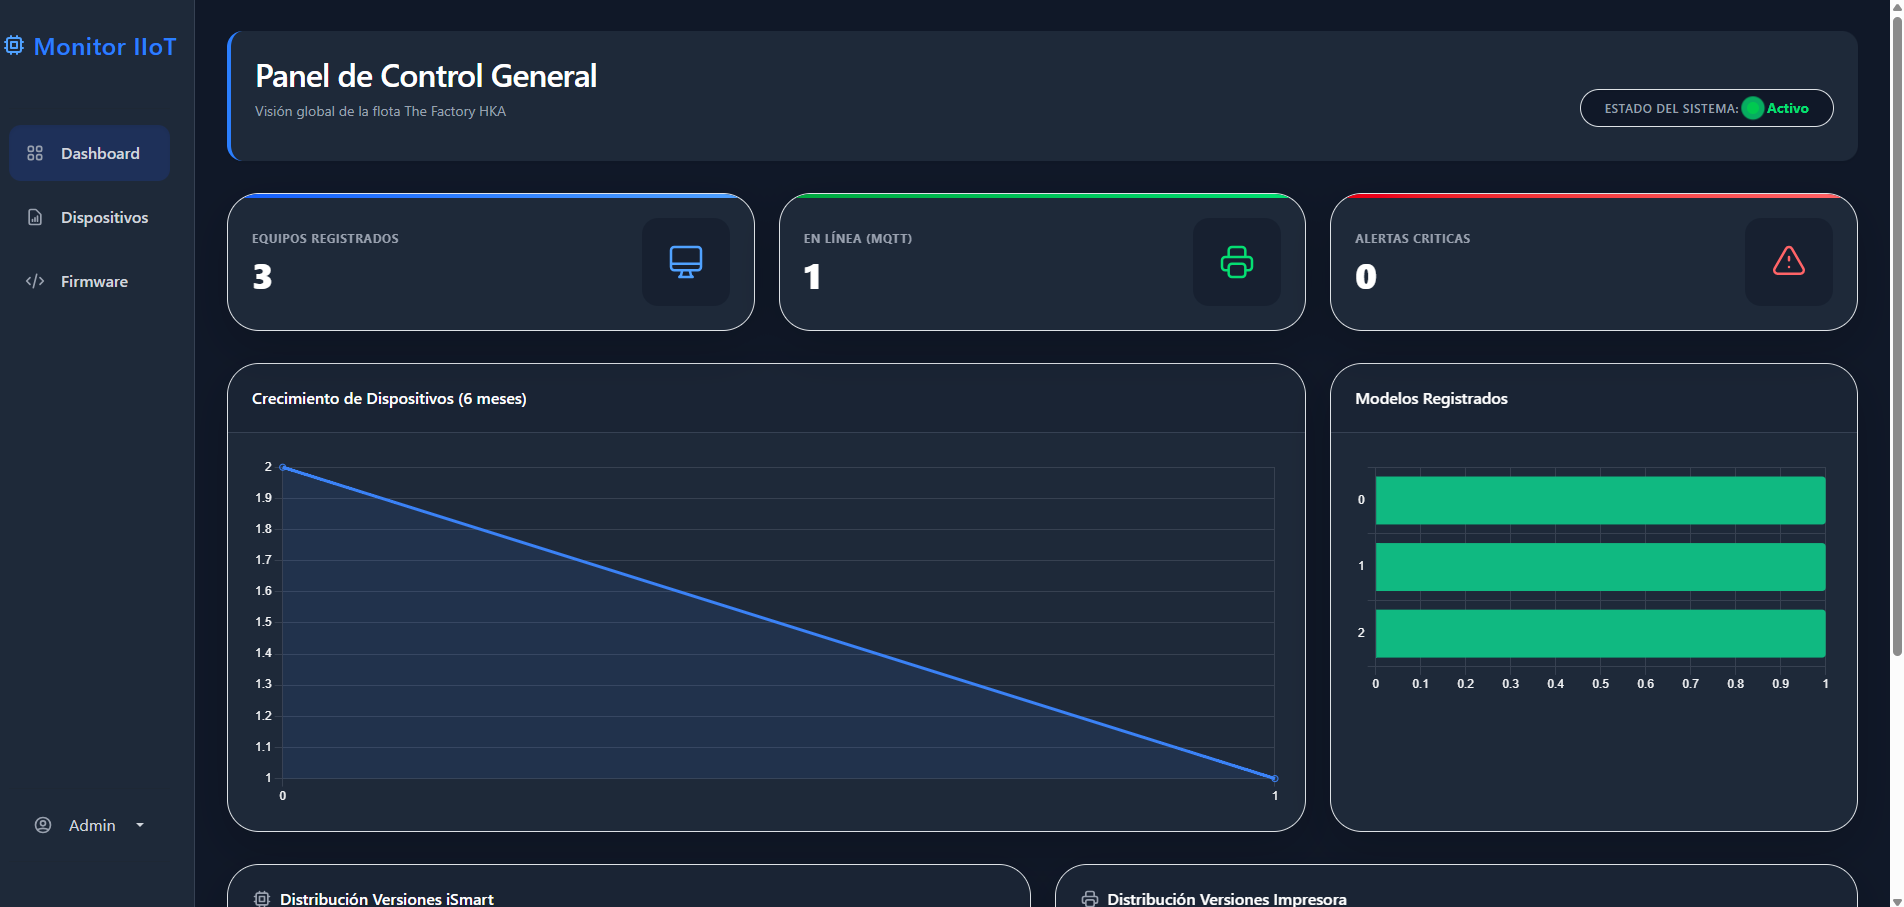
\includegraphics[width=0.95\textwidth]{Img/dashboard_tiempo_real.png}
    \caption{Panel de Control General (Dashboard) operando bajo arquitectura SPA reactiva.}
    \label{fig:dashboard_tiempo_real}
\end{figure}

\par Por su parte, la evaluación del módulo de auditoría de errores (véase la Figura \ref{fig:log_capture_error}) confirmó que el \textit{Worker} en Django intercepta y registra de forma independiente las variaciones lógicas del hardware \cite{Django_v5_Doc}. La captura documenta la transición exacta desde un estado normal (\texttt{0x60}) hacia un código de en medio de una transacción fiscal (\texttt{0x61}), correspondiente a la operación de imprimir una factura en la impresora fiscal \cite{TheFactoryHKA_Manual_Protocolos}.

\begin{figure}[htbp]
    \centering
    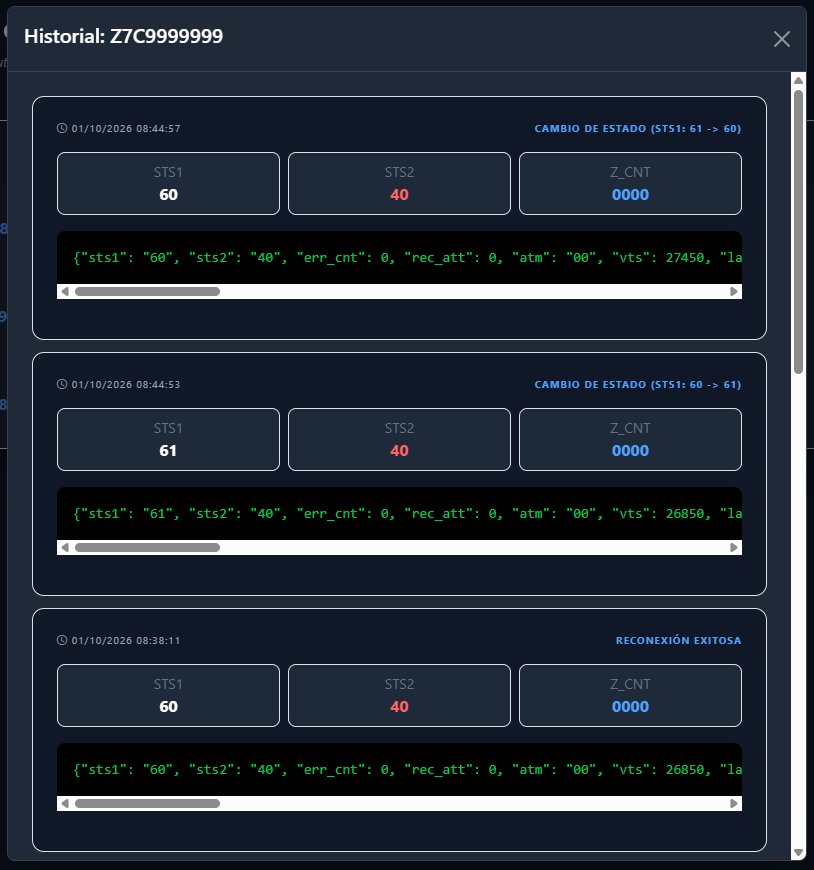
\includegraphics[width=0.75\textwidth]{Img/log_capture_error.png}
    \caption{Visualización en \texttt{Log Capture} de un cambio de estado de error mecánico (\texttt{0x48}).}
    \label{fig:log_capture_error}
\end{figure}

\section{Pruebas del Sistema de Actualización Remota (OTA)}
\label{sec:ota_resultados}

\par La validación de la actualización remota de firmware se dividió según el destino lógico del binario compilado: la autoactualización del gateway ESP32 o la reescritura del periférico fiscal \cite{Espressif_ESP_IDF_v552}.

\par El flujo completo de orquestación de la actualización remota de doble objetivo, desde la interfaz web hasta el reporte final, se sintetiza en la Figura \ref{fig:flujo_ota}.

\begin{figure}[htb]
\centering
\begin{tikzpicture}[>=latex', node distance=0.7cm,
    p/.style={rectangle, draw, rounded corners, fill=blue!10, text width=7.8cm, align=center, minimum height=0.8cm, font=\small},
    b/.style={rectangle, draw, rounded corners, fill=green!10, text width=5.6cm, align=center, minimum height=1.0cm, font=\scriptsize},
    d/.style={diamond, draw, fill=orange!15, aspect=3, align=center, font=\scriptsize},
    ar/.style={thick,->,>=stealth}]
    \node [p] (w) {El usuario presiona \say{Enviar Actualización} en la interfaz HTMX};
    \node [p, below=of w] (m) {Publicación MQTT del comando en \texttt{comandos/\{serial\}/ota}};
    \node [p, below=of m] (e) {Recepción en el ESP32 y activación de \texttt{ota\_en\_progreso}};
    \node [d, below=of e] (dec) {¿Destino del binario?};
    \node [b, below left=1.0cm and 0.2cm of dec] (gw) {\textbf{Gateway}: descarga HTTPS y escritura en la partición OTA inactiva};
    \node [b, below right=1.0cm and 0.2cm of dec] (pr) {\textbf{Impresora}: puente síncrono Chunk/ACK con verificación de \textit{checksum}};
    \node [p, below=3.0cm of dec] (v) {Verificación de integridad y reporte de estado a la interfaz web};
    \draw [ar] (w) -- (m);
    \draw [ar] (m) -- (e);
    \draw [ar] (e) -- (dec);
    \draw [ar] (dec) -- node[left, font=\scriptsize]{\texttt{ismart}} (gw);
    \draw [ar] (dec) -- node[right, font=\scriptsize]{\texttt{printer}} (pr);
    \draw [ar] (gw.south) |- (v.west);
    \draw [ar] (pr.south) |- (v.east);
\end{tikzpicture}
\caption{Diagrama de flujo de la orquestación de la actualización remota (OTA) de doble objetivo.}
\label{fig:flujo_ota}
\end{figure}

\subsection{Auto-actualización del Módulo Gateway (ESP32)}

\par Al seleccionar el objetivo \say{\texttt{ismart}} desde la plataforma web (véase la Figura \ref{fig:ota_mt_iot}), el MT-IoT recibió la orden por MQTT y activó la bandera de suspensión (\texttt{ota\_en\_progreso = true}) \cite{FreeRTOS_Kernel_Ref}. Las pruebas de descarga HTTPS verificaron la escritura en la partición OTA inactiva dentro del mapa de memoria de 4 MB \cite{Espressif_ESP_IDF_v552}. Se constató que la reducción de la frecuencia de la CPU a 80 MHz mediante \texttt{menuconfig} \cite{Espressif_Menuconfig} estabilizó la corriente consumida durante la descodificación criptográfica.

\begin{figure}[htbp]
    \centering
    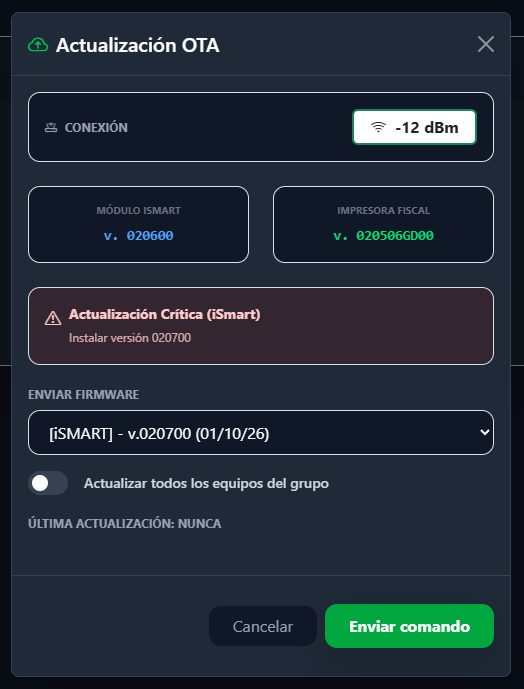
\includegraphics[width=0.55\textwidth]{Img/ota_mt_iot.png}
    \caption{Intermediación web desplegando una actualización de firmware crítica hacia el MT-IoT.}
    \label{fig:ota_mt_iot}
\end{figure}

\subsection{Puente Síncrono Heterogéneo de Reescritura de Firmware In Situ}

\par La operación de mayor complejidad no consistió en la carga de un archivo mediante HTTP, sino en la reescritura \textit{in situ} de la memoria del periférico fiscal a través de un puente síncrono heterogéneo que tradujo el flujo de un canal IP asíncrono al dominio determinista del bus local \cite{TheFactoryHKA_Manual_Protocolos}. El binario se transfirió por fragmentos de $1024$ bytes, cada uno de los cuales fue empaquetado con una cabecera de control de $4$ bytes (identificador de paquete, índice secuencial y longitud en $16$ bits) y un código de redundancia XOR calculado sobre los datos, conformando una trama robusta reenviable hasta un máximo de $3$ intentos con confirmación explícita (\texttt{ACK}) por parte del periférico. La ventana de trabajo se gestionó sobre un búfer circular de $1$~KB reutilizado cíclicamente en cada fragmento, de manera que la huella de memoria del proceso permaneció constante e independiente del tamaño del firmware, que ronda los $900$~KB.\\

\par La robustez frente a contingencias de red se evaluó desconectando arbitrariamente la interfaz Wi-Fi durante la transferencia. Ante la pérdida del canal, el firmware no reinicia la descarga desde el byte cero: reabre la conexión HTTP adjuntando la cabecera de rango \texttt{Range: bytes=<desplazamiento>-}, de forma que el servidor reanuda el envío exactamente en el fragmento donde se interrumpió. Esta estrategia de transferencia reanudable por fragmentos (\textit{HTTP Range Requests}) se sostuvo sobre un lazo de persistencia de hasta $5$ reintentos consecutivos, cuyo contador se reinicia cada vez que se confirma progreso real, garantizando que la operación sobreviva a cortes intermitentes de Wi-Fi o a reinicios transitorios del enlace. Adicionalmente, el sistema activa el lazo de reconexión inalámbrica (\texttt{WIFI\_EVENT\_STA\_DISCONNECTED}) y, al restablecerse el contacto con el \textit{Broker} MQTT, el dispositivo retorna a su estado operativo habitual sin bloqueos del microcontrolador.\\

\par La integridad del binario se garantizó por construcción: la secuencia de control se compone de una apertura de sesión (\texttt{0x07}), la ráfaga de paquetes de datos (\texttt{0x08}) y un cierre explícito (\texttt{0x09}) que el puente solo emite cuando el contador de bytes confirmados iguala la longitud total declarada por el servidor. En consecuencia, una transferencia parcial nunca llega a comprometerse en la memoria del periférico, y ante una nueva orden de actualización emitida desde la plataforma el proceso se reinicia desde el $0\%$ para preservar la coherencia absoluta del firmware. Con el propósito de no interferir con la máquina de estados fiscal, la reescritura se arbitró mediante la bandera de suspensión (\texttt{ota\_en\_progreso}) y el semáforo del bus (\texttt{spi\_bus\_mutex}), que ponen la rutina de sondeo en reposo mientras el puente ocupa el canal físico \cite{FreeRTOS_Kernel_Ref}.\\

\par Una vez confirmada la recepción de la totalidad de los bloques con verificación de redundancia local (LRC/Checksum), el periférico fiscal ejecuta un reinicio por hardware y consolida el nuevo firmware \cite{TheFactoryHKA_Manual_Protocolos}. Como se evidencia en la notificación flotante de la Figura \ref{fig:ota_printer_exito}, la interfaz web confirma el éxito de la operación mediante el mensaje: \say{Actualización Completada: El equipo Z7C9999999 actualizó printer con éxito}.

\begin{figure}[htbp]
    \centering
    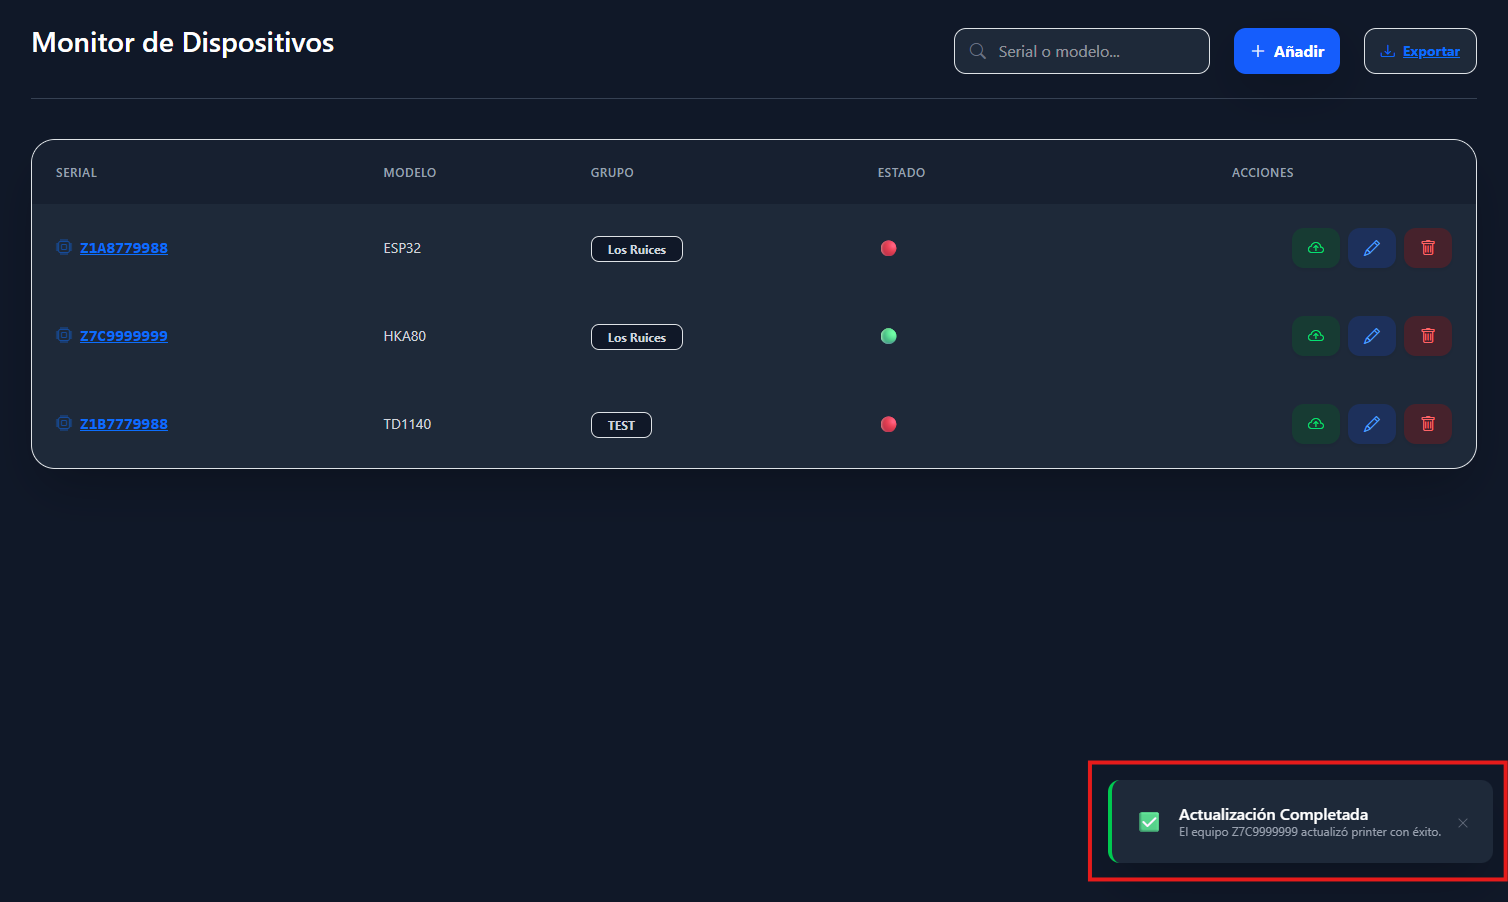
\includegraphics[width=0.85\textwidth]{Img/ota_printer_exito.png}
    \caption{Confirmación asíncrona en la interfaz web de actualización exitosa en la impresora fiscal.}
    \label{fig:ota_printer_exito}
\end{figure}

\section{Análisis de Rendimiento y Estabilidad Global del Sistema}

\par El análisis final de la arquitectura sistematiza la optimización de los recursos físicos del SoC ESP32 y la estabilidad del servidor de persistencia.

\subsection{Perfilado Formal de Memoria IRAM y DRAM}

\par La reingeniería aplicada mediante la utilidad \texttt{menuconfig} \cite{Espressif_Menuconfig} para liberar espacio en la memoria estática IRAM se evaluó comparando la ocupación de memoria antes y después de desactivar la aceleración por IRAM del \textit{stack} Wi-Fi \cite{Espressif_ESP_IDF_v552}. Los resultados del perfilado se organizan en la Tabla \ref{tab:perfilado_iram}.

\begin{table}[htbp]
\centering
\caption{Perfilado de recursos de memoria IRAM y DRAM en el SoC ESP32 ante optimizaciones de \texttt{menuconfig}.}
\label{tab:perfilado_iram}
\begin{tabularx}{\textwidth}{@{}>{\raggedright\arraybackslash}X >{\raggedright\arraybackslash}p{2.1cm} >{\raggedright\arraybackslash}p{1.7cm} >{\raggedright\arraybackslash}p{2.1cm} >{\raggedright\arraybackslash}p{2.2cm}@{}}
\toprule
\textbf{Estado del Firmware} & \textbf{IRAM Usada (Bytes)} & \textbf{IRAM (\%)} & \textbf{DRAM Usada (Bytes)} & \textbf{Ahorro Directo} \\
\midrule
1. Pila Completa (Wi-Fi IRAM Activo) & 102,751 & 78.39 \% & 37,852 & 0.00 \% (Crítico) \\
2. Reingeniería (Wi-Fi IRAM Inactivo) & 68,495 & 52.26 \% & 37,424 & \textbf{26.13 \%} \\
\midrule
\textbf{Margen Libre Resultante} & \textbf{62,577 B} & \textbf{47.74 \%} & \textbf{143,312 B} & --- \\
\bottomrule
\end{tabularx}
\end{table}

\par Las capturas de perfilado obtenidas en el entorno de desarrollo (Figura \ref{fig:iram_78} y Figura \ref{fig:iram_52}) confirman una reducción efectiva de $34,256 \text{ Bytes}$ en la IRAM \cite{Espressif_Menuconfig}. Este espacio libre resultó indispensable para reservar el búfer dinámico necesario durante las tareas de actualización OTA.

\begin{figure}[htbp]
    \centering
    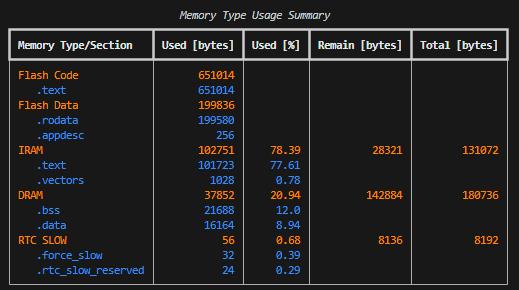
\includegraphics[width=0.75\textwidth]{Img/iram_78.png}
    \caption{Perfilado de memoria inicial revelando ocupación crítica de IRAM ($78.39\%$).}
    \label{fig:iram_78}
\end{figure}

\begin{figure}[htbp]
    \centering
    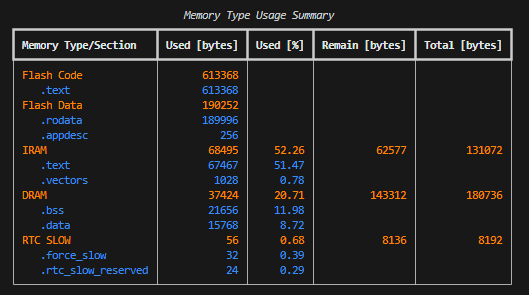
\includegraphics[width=0.75\textwidth]{Img/iram_52.png}
    \caption{Ocupación de IRAM optimizada al $52.26\%$ tras deshabilitar aceleración Wi-Fi.}
    \label{fig:iram_52}
\end{figure}

\subsection{Perfilado Térmico y Energético del Subclocking (80 MHz)}

\par La reducción deliberada de la frecuencia del núcleo del SoC, desde el máximo nominal de $240$~MHz hasta $80$~MHz, se evaluó no solo como una medida de estabilidad funcional, sino como una decisión de gestión térmica y energética. La potencia dinámica disipada por un circuito CMOS se rige por la Ecuación \ref{eq:potencia_dinamica}:

\begin{equation}
P_{din} = C_{ef} \cdot V_{dd}^{2} \cdot f
\label{eq:potencia_dinamica}
\end{equation}

\par donde $C_{ef}$ es la capacitancia efectiva conmutada, $V_{dd}$ la tensión de alimentación del núcleo y $f$ la frecuencia de operación. Dado que en el ESP32 la tensión del núcleo es regulada internamente y permanece prácticamente constante, la frecuencia constituye la única variable de control directo sobre el consumo dinámico; en consecuencia, reducir $f$ en un factor de $3$ (de $240$ a $80$~MHz) contrae la potencia dinámica en la misma proporción. Esta reducción se traduce de forma directa en la disipación térmica, ya que el salto térmico entre la unión y el ambiente sigue la Ecuación \ref{eq:salto_termico}:

\begin{equation}
\Delta T_{j-a} = P \cdot R_{\theta j-a}
\label{eq:salto_termico}
\end{equation}

\par con $R_{\theta j-a}$ como la resistencia térmica unión-ambiente, constante para un encapsulado y una placa dadas. Al reducirse $P$, el gradiente $\Delta T_{j-a}$ disminuye en la misma proporción, rebajando la temperatura de operación del silicio y, con ello, el estrés térmico acumulado en régimen continuo. La Tabla \ref{tab:underclocking} sintetiza el compromiso entre frecuencia, potencia dinámica relativa y suficiencia criptográfica.\\

\begin{table}[htbp]
\centering
\caption{Compromiso térmico-energético del subclocking del SoC ESP32.}
\label{tab:underclocking}
\begin{tabularx}{\textwidth}{@{}>{\raggedright\arraybackslash}p{3.0cm} >{\raggedright\arraybackslash}X >{\raggedright\arraybackslash}X >{\raggedright\arraybackslash}X@{}}
\toprule
\textbf{Frecuencia del CPU} & \textbf{Potencia Dinámica ($P \propto f$)} & \textbf{Salto Térmico ($\Delta T \propto P$)} & \textbf{Suficiencia Criptográfica (AES)} \\
\midrule
$240$~MHz (nominal) & $1.00$ (referencia) & $1.00$ (referencia) & Sí, sobredimensionado \\
$160$~MHz & $0.67$ & $0.67$ & Sí \\
$80$~MHz (adoptado) & $0.33$ & $0.33$ & Sí (handshake TLS: $45$~ms $< 100$~ms) \\
\bottomrule
\end{tabularx}
\end{table}

\par El aspecto crítico que habilita esta reducción es la presencia del acelerador criptográfico AES por hardware del ESP32: la operación intensiva de cifrado no se ejecuta en el núcleo, sino en un bloque dedicado, por lo que la frecuencia del CPU solo debe ser suficiente para alimentar y orquestar dicho acelerador. Bajo esta condición, el $80$~MHz demostró sostener el handshake TLS en $45$~ms, holgadamente dentro de la ventana de tolerancia de $100$~ms (véase la Tabla \ref{tab:latencias}). El efecto observable sobre la alimentación fue la estabilización de la corriente durante las ráfagas criptográficas: al no exigirse al núcleo picos de conmutación, la demanda instantánea se vuelve más uniforme, reduciendo las transitorias de corriente ($di/dt$) y la solicitación sobre el regulador de la placa. En términos de gestión térmica, la caída del salto térmico a un tercio del valor nominal se traduce en una operación más fría y en una menor degradación por ciclado térmico, elevando la decisión de subclocking del plano puramente funcional al del diseño térmico y energético del nodo.

\subsection{Trazabilidad y Estabilidad de Almacenamiento en Servidor SQLite}

\par En el nivel de gestión en la nube, se midió el crecimiento de la base de datos relacional SQLite (\texttt{db.sqlite3}) sometida a ráfagas de telemetría continua \cite{Django_v5_Doc}. La implementación de la rutina de depuración automática ($\texttt{fecha\_limite} = \texttt{timezone.now()} - \texttt{timedelta(days=90)}$) dentro del \textit{Worker} demostró ser efectiva. Las pruebas de estrés con un histórico simulado de $10,000$ registros confirmaron que la depuración asíncrona purga los registros obsoletos sin bloquear las consultas de la interfaz web, manteniendo la tasa de respuesta en búsquedas indexadas por serial por debajo de los $12 \text{ ms}$ \cite{Django_v5_Doc}.\\

\par La trazabilidad se materializó sobre dos entidades relacionales: el dispositivo fiscal, identificado de forma unívoca por su número de serie, y su bitácora de eventos (\texttt{LogDispositivo}), vinculada mediante clave foránea y ordenada cronológicamente de forma descendente. El \textit{Worker} asíncrono \texttt{listen\_mqtt.py} se suscribe a los tópicos de telemetría y de alertas de conexión, y por cada trama recibida no almacena un único registro, sino que compara el estado entrante contra el último estado persistido y descompone la diferencia en eventos atómicos e independientes: cambios de estado lógico (\texttt{STS1}), transiciones de error mecánico (\texttt{STS2}), cortes de reporte Z, emisión de facturas, reconexiones y actualizaciones de firmware (véase el Código \ref{code:listen_mqtt}). Esta descomposición por evento, evaluada ante ráfagas de telemetría, demostró preservar la granularidad de la auditoría sin degradar el desempeño de escritura.\\

\par La eficiencia de las consultas se sostuvo sobre dos decisiones de diseño verificadas empíricamente. En primer lugar, el acceso a la vista de auditoría emplea la carga diferida de relaciones mediante \texttt{select\_related} y \texttt{prefetch\_related} sobre el conjunto ordenado de registros, reduciendo el problema de consultas N+1 a un número constante de accesos a la base de datos. En segundo lugar, la búsqueda por serial utiliza coincidencia indexada (\texttt{serial\_\_icontains}) que, combinada con el ordenamiento por fecha, mantiene la latencia de recuperación por debajo de los $12$~ms incluso con el histórico completo cargado. La rutina de retención de $90$ días, además, acota el volumen histórico de forma continua, de modo que la profundidad de la bitácora permanece estable en el tiempo y las consultas conservan su tasa de respuesta ante ráfagas sostenidas de eventos \cite{Django_v5_Doc}.